% !TEX TS-program = pdflatexmk
\documentclass[12pt]{article}

% Layout.
\usepackage[top=1in, bottom=0.75in, left=1in, right=1in, headheight=1in, headsep=6pt]{geometry}

% Fonts.
\usepackage{mathptmx}
\usepackage[scaled=0.86]{helvet}
\renewcommand{\emph}[1]{\textsf{\textbf{#1}}}

% Misc packages.
\usepackage{amsmath,amssymb,latexsym}
\usepackage{graphicx,hyperref}
\usepackage{array}
\usepackage{xcolor}
\usepackage{multicol}
\usepackage{tabularx,colortbl,booktabs,xparse}
\usepackage{enumitem}

\usepackage{tikz}
\usetikzlibrary{calc, positioning}

% Rotation: \rot[<angle>][<width>]{<stuff>}
\NewDocumentCommand{\rot}{O{45} O{1em} m}{\makebox[#2][l]{\rotatebox{#1}{#3}}}%

\usepackage{fancyhdr}
\pagestyle{fancy} 
\lhead{\large\sf\textbf{MATH F113X: Voting Theory}}
\chead{\large\sf\textbf{lecture notes}}
\rhead{\large\sf\textbf{Day 2}}

\begin{document}
\begin{enumerate}
%\item Review from Voting Theory Day 1\\
%	\begin{enumerate}
%	\item majority winner versus plurality winner
%	\vfill
%	\item Condorcet winner
%	\vfill
%	\item What can go wrong with plurality voting?
%	\vfill
%	\end{enumerate}
%Recall the (slightly modified!) example from Day 1:
%
%Eleven Alaskans are asked to vote on the ``best" of four Alaskan villages.\\
%
%Villages: \textbf{A}dak, \textbf{B}ettles, \textbf{C}hevak, \textbf{D}iomede\\
%
%\begin{tabular}{l || c |c|c|c|c}
%\# votes&3&4&2&1&1\\
%\hline
%1st choice&A&B&C&C&D\\
%2nd choice&C&C&D&B&C\\
%3rd choice&B&D&B&A&B\\
%4th choice&D&A&A&D&A\\
%\end{tabular}
%
%\vfill
%
%\item \textbf{Insincere Voting}
%
%\vfill
%\item Remedy for insincere voting?
\newpage

\item Problems with plurality voting?

\vspace{1in}
\item Instant Runoff Voting (IRV), also known as \hrulefill
\vspace{2.5in}


\item With four candidates, how many rounds of IRV? (Max? Min?)
\vspace{1in}

\item Find the winner using IRV for the preference schedule below.\\
\begin{tabular}{l || c |c|c|c|c}
\# votes&3&4&2&1&1\\
\hline
1st choice&A&B&C&C&D\\
2nd choice&C&C&D&B&C\\
3rd choice&B&D&B&A&B\\
4th choice&D&A&A&D&A\\
\end{tabular}

\vfill
\newpage

\item (Example 7) Find the winner using IRV for the preference schedule below.\\
\begin{tabular}{l || c |c|c|c|}
\# votes&37&22&12&29\\
\hline
1st choice&Adams&Brown&Brown&Carter\\
2nd choice&Brown&Carter&Adams&Adams\\
3rd choice&Carter&Adams&Carter&Brown\\

\end{tabular}

\vfill

\item What can go wrong with IRV?
	\begin{enumerate}
	\item Fail to pick the Condorcet Winner (See example 6 in your text.)
	\item Fails the \emph{Monotonicity Criterion}:
	
	\vfill
	\end{enumerate}
	
\item (Example 7 again)\\

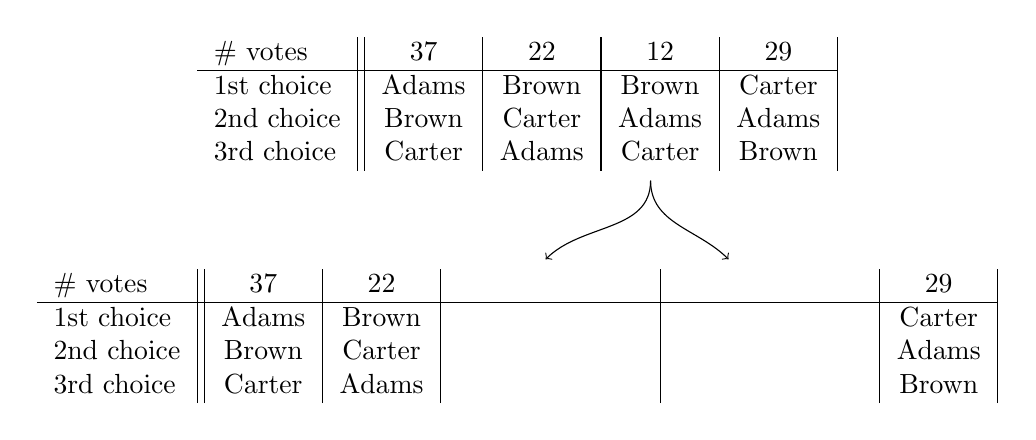
\begin{tikzpicture}
\node (first) at (0,0){
\begin{tabular}{l || c |c|c|c|}
\# votes&37&22&12&29\\
\hline
1st choice&Adams&Brown&Brown&Carter\\
2nd choice&Brown&Carter&Adams&Adams\\
3rd choice&Carter&Adams&Carter&Brown\\
\end{tabular}
};

\path node[below = of first] (last)
{\begin{tabular}{l || c |c|c|c|c|}
\# votes&37&22&\quad\hspace{2cm}\quad&\quad\hspace{2cm}\quad&29\\
\hline
1st choice&Adams&Brown&&&Carter\\
2nd choice&Brown&Carter&&&Adams\\
3rd choice&Carter&Adams&&&Brown\\
\end{tabular}
};

\draw[->] (first.330) to[out = 270, in = 45] (last.70);% the node.# notation is using an angle measure around the node!
\draw[->] (first.330) to[out = 270, in = 180-45] (last.20);

\end{tikzpicture}
\vfill
\end{enumerate}
\end{document}